\chapter{FUNDAMENTAÇÃO TEÓRICA}\label{cap:fundamentacao-teorica}


Detalhar o overview da fundamentação teórica com a motivação principal
de todas as explicações


\section{Segmentação interativa de imagens}\label{sec:segmentacao-interativa}

A segmentação interativa de imagens é um processo de divisão de uma
imagem digital em várias partes ou regiões, geralmente para tornar a
imagem mais fácil de analisar e processar~\cite{ramadan2020survey}. Este processo é `interativo'
porque envolve a entrada do usuário para ajudar a orientar ou refinar
o processo de segmentação.

\begin{figure}[h!]
        \captionsetup{width=12cm}
		\Caption{\label{fig:interactive-segmentation}
          O usuário marca anotações do fundo e do objeto a ser
          segmentado, então a segmentação interativa é realizada.
        }
		\centering
		\UFCfig{}{\fbox{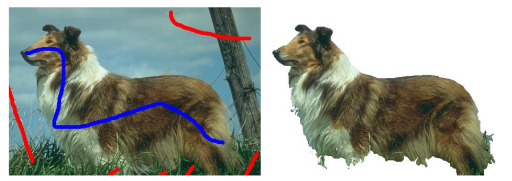
\includegraphics[width=12cm]{figuras/interactive-segmentation-2008}}}{\Fonte{\cite{duchenne2008segmentation}}}
\end{figure}
\FloatBarrier{}

De acordo com a figura~\ref{fig:interactive-segmentation}, na
segmentação interativa de imagens, o usuário pode selecionar regiões
de interesse, definir marcadores ou fazer anotações na imagem. Essas
entradas do usuário são então usadas para informar o algoritmo de
segmentação sobre como dividir a imagem. Por exemplo, o usuário pode
desenhar uma linha ao redor de um objeto de interesse, e o algoritmo
de segmentação irá então tentar dividir a imagem de tal forma que o
objeto de interesse seja isolado em sua própria região.

Este tipo de segmentação de imagem é útil em uma variedade de
aplicações, incluindo processamento de imagens médicas, visão
computacional, reconhecimento de padrões e muitos outros campos onde é
útil poder dividir uma imagem em regiões distintas com base em
critérios definidos pelo usuário.

\section{Aprendizado semi-supervisionado vs.\ transdução}\label{sec:teorica-aprendizado-semi-supervisionado}

Existem três principais categorias de aprendizado de máquina:
aprendizado supervisionado, aprendizado não-supervisionado e
aprendizado semi-supervisionado. No aprendizado supervisionado durante
a etapa de treinamento existe uma base de dados totalmente rotulada,
no aprendizado não-supervisionado não é disponibilizado nenhum
rotulamento dos dados. Enquanto isso, o aprendizado
semi-supervisionado está entre essas duas categorias.

O aprendizado semi-supervisionado é um método de aprendizado de máquina
que envolve o uso de um grande volume de dados não rotulados e um
pequeno volume de dados rotulados para treinar modelos de aprendizado
de máquina.

Formalmente, pode-se definir o aprendizado semi-supervisionado da seguinte maneira:

\begin{quote}
  Dado um conjunto de dados de treinamento
  $ \mathbf{X} = \{\vec{x_1}, \vec{x_2}, \ldots, \vec{x_n}\} $, tal que $ \vec{x_n} \in \mathbb{R}^d $,
  onde apenas um subconjunto  $ \vec{Y} = \{y_1, y_2, \ldots , y_m\} $ em que $ (m < n) $ tem rótulos
  correspondentes, o objetivo do aprendizado semi-supervisionado é usar
  tanto o conjunto de dados rotulado quanto o não rotulado para aprender
  a função $ f: \mathbf{X} \rightarrow \vec{Y} $ que pode prever o rótulo $ y $ para um novo
  exemplo $ \vec{x} $.
\end{quote}

O aprendizado semi-supervisionado é baseado na suposição de que os
dados não rotulados podem fornecer informações adicionais que podem
ser usadas para melhorar a precisão do modelo de aprendizado de
máquina. Isso é feito através de várias técnicas, como a propagação de
rótulos, onde os rótulos são propagados dos dados rotulados para os
dados não rotulados, ou a aprendizagem auto-supervisionada, onde o
modelo é treinado para prever partes dos dados a partir de outras
partes.

Por outro lado, existe um diferente tipo de aprendizado
semi-supervisionado que não realiza a etapa de estimar a função $ f
$. Algoritmos que estimam essa função são descritos como indutivos,
pois após o treinamento, para classificar novos dados, realizam uma
inferência por indução ao aplicar a função estimada.

Em contraponto, existem algoritmos que não estimam tal função e apenas
realizam a inferência direta entre os dados rotulados disponíveis e os
não rotulados. Isso é chamado de transdução e um algoritmo bem
conhecido com essa característica é o classificador K-NN.\@ Na
figura~\ref{fig:induction-vs-transduction} a seguir, é ilustrado as
diferenças entre transdução e indução no processo de aprendizagem:


\begin{figure}[h!]
        \captionsetup{width=12cm}
		\Caption{\label{fig:induction-vs-transduction}
          No aprendizado transdutivo, a inferência em novos exemplos
          ocorre de maneira direta.
        }
		\centering
		\UFCfig{}{\fbox{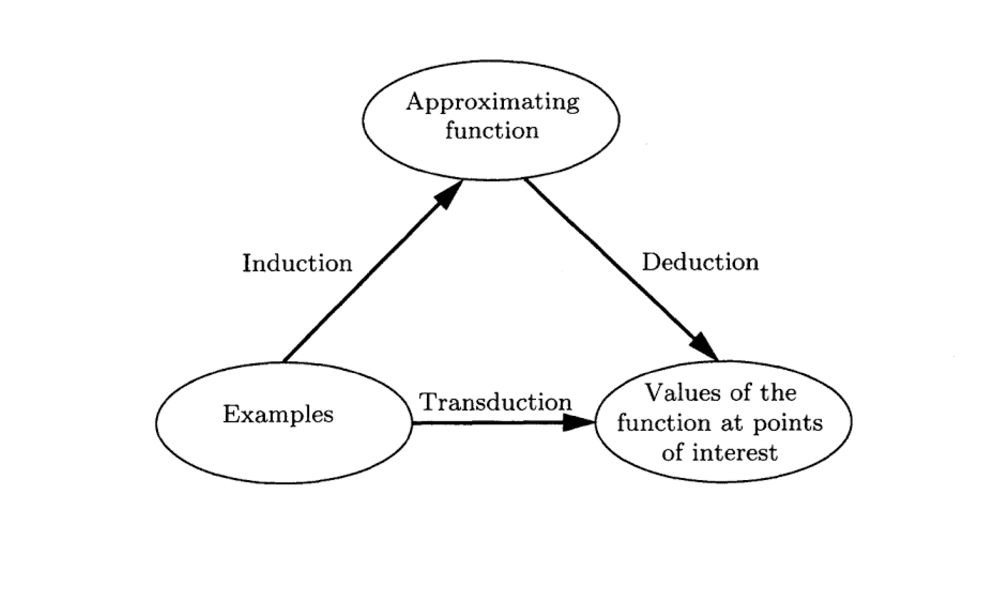
\includegraphics[width=12cm]{figuras/induction_vs_transduction}}}{\Fonte{\cite{vapnik1995}}}
\end{figure}


No texto~\cite{vapnik2006semi}, o criador do famoso algoritmo SVM,
estabelece uma profunda formalização dos problemas de aprendizado
semi-supervisionado e inferência transdutiva. No final do texto, ele declara
algumas reflexões sobre a solução de problemas em aprendizagem de
máquina. Em uma delas, ele diz que ao resolver um problema, não tente
resolve o problema geral como um passo intermediário, tente obter a
resposta que você precisa, mas não a mais geral. Por fim, um Vapnik
deixa uma sugestão relevante:


\begin{displayquote}

  Do not estimate a function if you need to estimate values at given
  points. (Try to perform transduction, not induction.)

\end{displayquote}

Em tradução-livre: \blockquote{Não estime uma função se você precisa estimar
os valores em dados pontos. (Tente executar transdução, não
indução)}. Essa sugestão é uma evidência que reforça a motivação
deste trabalho. Ao desenvolver um algoritmo transdutivo pra
segmentação de imagens de maneira assistida, não é estimado uma função
geral como um passo intermediário, mas a segmentação é realizada
diretamente baseado nas rotulações iniciais que o usuário forneceu.


\section{Superpixels}\label{sec:teorica-superpixel}

Superpixels fazem parte de um grupo de algoritmos de clusterização em
processamento de imagens que ganhou popularidade nos últimos anos na
comunidade de visão computacional~\cite{SuperpixelSurvey2020}. Em vez
de processar uma imagem pixel por pixel, agrupa-se pixels vizinhos
semelhantes em uma entidade maior, conhecida como superpixel.

O conceito de superpixels foi introduzido para superar as limitações
do processamento pixel a pixel, que não leva em consideração a
estrutura global da imagem. Os superpixels, por outro lado, mantêm a
estrutura da imagem e reduzem a complexidade do processamento de
imagens, tornando-o mais eficiente.

Os superpixels são formados com base na similaridade dos pixels em
termos de cor, intensidade e localização na imagem. Eles são usados em
uma variedade de aplicações, incluindo segmentação de imagem,
rastreamento de objetos, reconhecimento de objetos, entre outros.

Em resumo, os superpixels são uma técnica eficaz para simplificar a
representação de uma imagem e aumentar a eficiência do processamento
de imagens, mantendo a informação visual importante.

Atualmente, já é possível encontrar muitas técnicas baseado em
superpixels com diferentes características, complexidade
computacionais, eficiência e método. No
artigo~\cite{SuperPixelBenchmark2017}, é realizado um benchmark com 15
algoritmos superpixels categorizados em três grupos: basedo em grafos,
baseado em otimização de gradiente e baseado em análise de
textura. Nesse trabalho, é selecionado um dos mais simples: \gls{SLIC}.

\subsection{SLIC}\label{sec:teorica-superpixel-slic}


O algoritmo \gls{SLIC} é um método para
a segmentação de imagens baseado em superpixel, é um dos mais simples
e pode ser visto como uma variação do algoritmo k-means expandindo o
espaço euclidiano ao incluir também o espaço de cores. Ele divide uma
imagem em segmentos menores, chamados superpixels, que compartilham
características semelhantes, como cor e textura.

Uma explicação passo-a-passo de como o SLIC funciona pode ser entendida
dessa maneira:

\begin{algorithm}[h!]
	\SetSpacedAlgorithm{}
	\caption{\label{alg:slic} SLIC}
	\Entrada{Imagem a ser segmentada}
    \Resultado{Matriz de superpixels}
	\Inicio{
      \begin{enumerate}

      \item \textbf{Inicialização}: O algoritmo começa selecionando alguns pixels na
        imagem como centros de superpixels. Esses centros são espaçados
        uniformemente pela imagem;

      \item \textbf{Atribuição}: Em seguida, para cada pixel na imagem, o algoritmo
        calcula a distância entre esse pixel e todos os centros de
        superpixels. A distância é calculada com base na cor (ou intensidade
        de cinza para imagens em preto e branco) e na proximidade espacial. O
        pixel é então atribuído ao superpixel cujo centro está mais próximo;

      \item \textbf{Atualização}: Depois que todos os pixels foram atribuídos a um
        superpixel, o algoritmo recalcula os centros de superpixels como a
        média de todos os pixels dentro de cada superpixel;

      \item O processo de atribuição e atualização é repetido várias vezes
        até que o algoritmo alcance a condição de convergência, ou seja, até
        que os centros de superpixels parem de mudar significativamente;

      \item O resultado final é uma segmentação da imagem em superpixels, onde
        cada superpixel é um grupo de pixels com características semelhantes.
    \end{enumerate}
   }
\end{algorithm}



Uma execução do SLIC é possível de ser visualizada a seguir:

\begin{figure}[h!]
        \captionsetup{width=12cm}
		\Caption{\label{fig:slic}
          Execução do algoritmo SLIC na fotografia de um gato.
        }
		\centering
		\UFCfig{}{\fbox{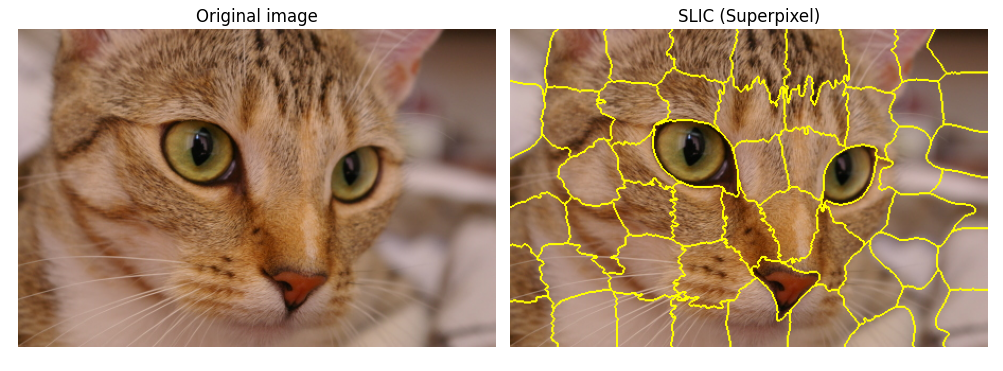
\includegraphics[width=12cm]{figuras/slic}}}{\Fonte{\fontefigura}}
\end{figure}


\section{Geração de redes complexas}\label{sec:teorica-redes-complexas}

Redes complexas são grafos de alta complexidade. Existem variados
algoritmos para geração de redes complexas
~\cite{ComplexNetworksSurvey2007}. Redes complexas podem ser usadas
como um domínio de dados para realizar tarefas como classificação de
imagens~\cite{ComplexNetworksImageClassification2015}, segmentação de
imagens, identificação de comunidades e também extração de
características~\cite{JarbasComplexNetworks2020}.

Neste trabalho, o uso de redes complexas é realizado de uma maneira
acoplada ao algoritmo de clusterização inicial da imagem (superpixel). Nesse
cenário, cada superpixel gerado na imagem é um vértice e as arestas
são gerados baseado na vizinhança.

Apesar de considerar o tema como redes complexas, esse cenário em
particular gera um grafo planar pela maneira como as arestas são
criadas. Por outro lado, seria possível também modificar a geração da
rede complexa para considerar as arestas do grafo baseado num raio
parametrizado de superpixel em relação a um \textit{treshrold} e
selecionar as k-nn similares como arestas válidas.

Essa etapa de geração da rede complexa é crucial para a execução da
dinâmica coletiva explorada na seção~\ref{sec:teorica-lcu}. Um dos
pontos centrais desse trabalho. Na figura~\ref{fig:complex-networks},
um exemplo de geração de rede complexa é apresentado conectado com a
ilustração~\ref{fig:slic}, ao executar o algoritmo SLIC.\@

\begin{figure}[t]
        \captionsetup{width=12cm}
		\Caption{\label{fig:complex-networks}
          Geração de rede complexa baseado nos superpixels.
        }
		\centering
		\UFCfig{}{\fbox{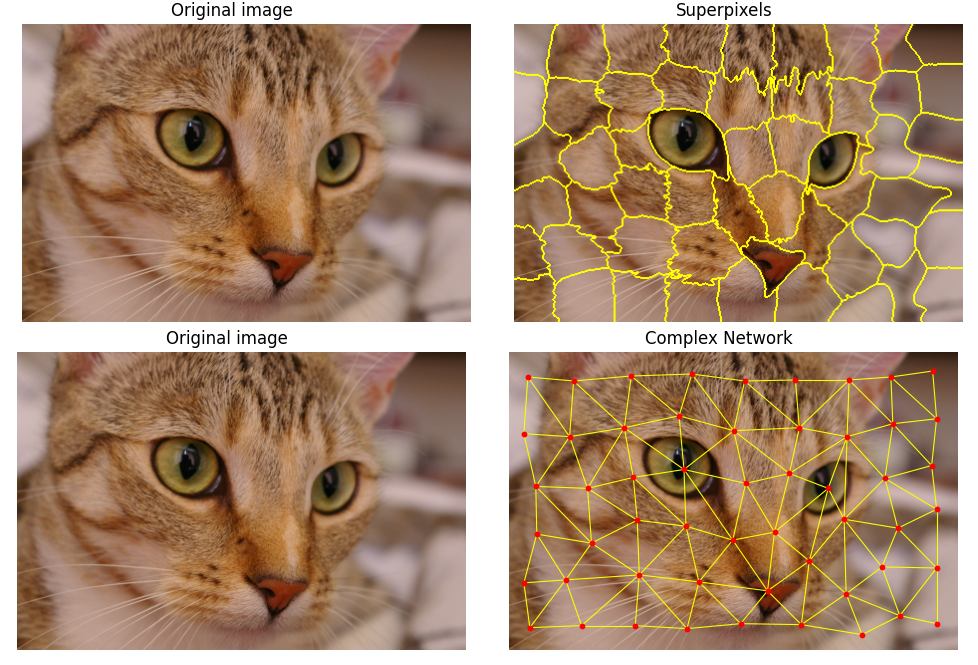
\includegraphics[width=12cm]{figuras/complex-networks}}}{\Fonte{\fontefigura}}
\end{figure}
\FloatBarrier{}

\section{Extração de características}\label{sec:extracao-caracteristicas}

\subsection{Matriz de co-ocorrências}\label{sec:teorica-matriz-co-ocorrencia}

O método de extração de características da matriz de co-ocorrências é
uma técnica utilizada em processamento de imagem e visão computacional
para extrair características texturais de uma imagem~\cite{matrizcoocorrencia2017}.

Formalmente, uma matriz de co-ocorrência C é definida sobre uma imagem
I, para um deslocamento $\Delta x, \Delta y$, como:

\begin{equation}\label{eq:comatrix}
  C_{\Delta x, \Delta y}(i,j) = \sum_{x=1}^n\sum_{y=1}^m
  \begin{cases} 1, & \text{if }I(x,y)=i\text{ e }I(x+\Delta x, y+\Delta y)=j
               \\ 0, & \text{caso contrário}
  \end{cases}
\end{equation}

Na equação~\ref{eq:comatrix} $C_{\Delta x, \Delta y}(i,j)$ é o número de vezes
que o par de pixels com intensidades i e j ocorre em dois pixels
separados pelas distâncias (horizontal e vertical) na imagem I.

A matriz de co-ocorrência é tipicamente normalizada dividindo cada
elemento pelo número total de pares de pixels na imagem, resultando em
uma matriz de probabilidade de co-ocorrência.

A partir desta matriz, várias características texturais podem ser
extraídas, como contraste, correlação, energia e homogeneidade. Estas
características podem ser usadas para tarefas como classificação de
textura, segmentação de imagem, entre outros.

\subsection{Filtros de gabor}\label{sec:filtros-gabor}

Escrever sobre métodos de extração de característica via filtros de gabor.

\section{Métricas de similaridade}\label{sec:teorica-metricas-de-similaridade}

A ser escrito: distância euclidiana, distância manhattan, distância
jaccard (?), métrica de similaridade exponencial $\exp(\dfrac{-d}{s})$

\section{LCU}\label{sec:teorica-lcu}

O algoritmo \gls{LCU} foi desenvolvido por um
brasileiro~\cite{VerriNetworkUnfoldingMap2018}, é uma dinâmica
coletiva baseado em propagação de rótulos numa rede complexa. Essa
dinâmica coletiva é modelada como um sistema dinâmico com geração de
partículas de rotulação nas suas fontes (os vértices rotulados).

Esse algoritmo possuem critérios de sobrevivência das particulas
inspirado em comportamentos da natureza e sociedade. Por exemplo, o
hiperparâmetro $ \lambda $ do algoritmo denota um fator entre 0 e 1 de
competitividade entre as partículas, tornando a sobrevivência delas
mais difícil ao percorrer o grafo. Embora as partículas nasçam nos
vértices, a competição por dominação acontece nas arestas. No final, o
vértice será marcado com o novo rótulo baseado no tipo de partícula
que mais conseguiu dominar arestas desse vértice.

Nesse caso particular, a implementação proposta é ligeiramente
diferente da proposta originalmente, pois a rede complexa no cenário
que o autor propõe as arestas não possuem peso. A modificação é
realizada para incluir a similaridade de imagem entre dois
superpixels, dessa maneira é criado um fator de aumento da
probabilidade das partículas visitarem os nós mais promissores. Como
discutido na seção
~\ref{sec:teorica-aprendizado-semi-supervisionado}, esse cenário de
aprendizado é semi-supervisionado transdutivo: poucos rótulos estão
disponíveis e nenhuma função de inferência é estimada. A inferência
acontece diretamente entre os pontos rótulados e os não-rotulados.


\begin{figure}[!h]
        \captionsetup{width=12cm}
		\Caption{\label{fig:lcu-partial}
          Rede complexa preparada com anotação parcial para execução do \gls{LCU}
        }
		\centering
		\UFCfig{}{\fbox{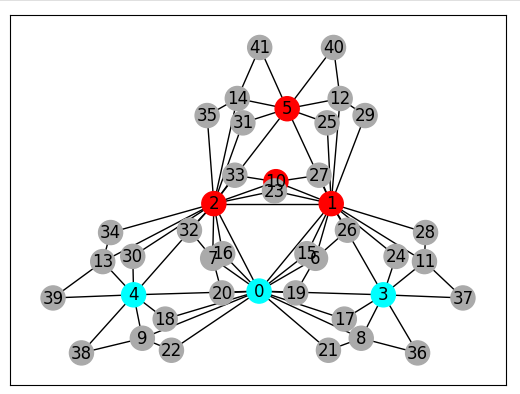
\includegraphics[width=12cm]{figuras/lcu-partial}}}{\Fonte{\fontefigura}}
\end{figure}
\FloatBarrier{}

\begin{figure}[!h]
        \captionsetup{width=12cm}
		\Caption{\label{fig:lcu-done}
          Execução do \gls{LCU} finalizada.
        }
		\centering
		\UFCfig{}{\fbox{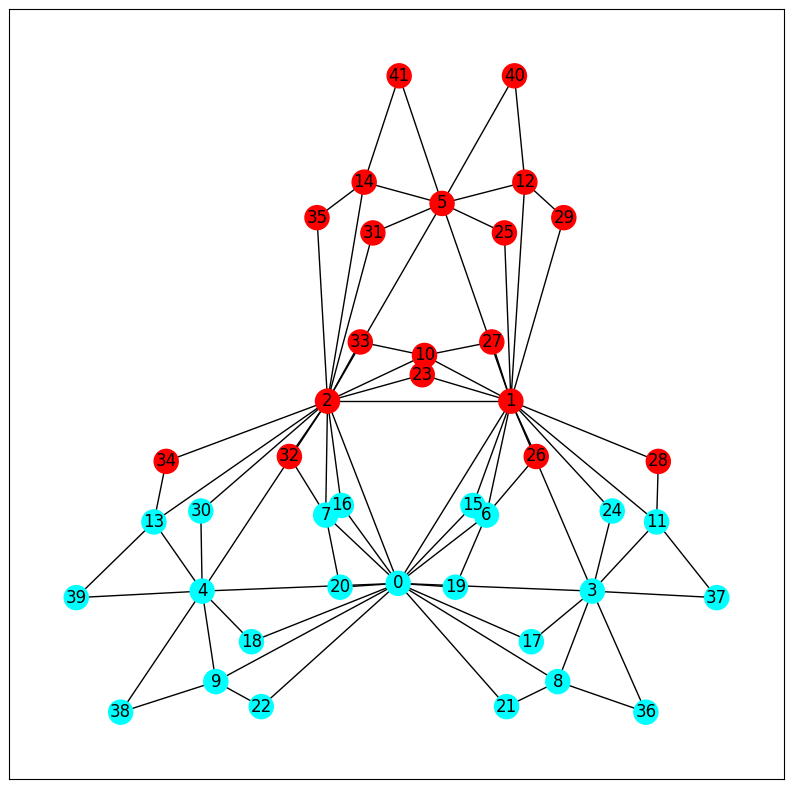
\includegraphics[width=12cm]{figuras/lcu-done}}}{\Fonte{\fontefigura}}
\end{figure}
\FloatBarrier{}

Nas figuras~\ref{fig:lcu-partially-annotated} e~\ref{fig:lcu-done} é
possível ver a execução do algoritmo numa rede complexa densa
aleatória, no final da execução os rótulos são propagados
semanticamente baseado na disputa entre as partículas.


\section{EGSIS}\label{sec:teorica-egsis}

A ser escrito, algoritmo agregador que une todas as partes.
